\documentclass[a5paper, 10pt]{article}

% Текст
\usepackage[utf8]{inputenc} % UTF-8 кодировка
\usepackage[russian]{babel} % Русский язык
\usepackage{indentfirst} % красная строка в первом параграфе в главе
% Отображение страниц
\usepackage{geometry} % размеры листа и отступов
\usepackage{listings}
\usepackage{color}

\usepackage{float}
\floatplacement{figure}{H}

\geometry{
	left=12mm,
	top=25mm,
	right=15mm,
	bottom=17mm,
	marginparsep=0mm,
	marginparwidth=0mm,
	headheight=10mm,
	headsep=7mm,
	nofoot}
\usepackage{afterpage,fancyhdr} % настройка колонтитулов
\pagestyle{fancy}
\fancypagestyle{style}{ % создание нового стиля style
	\fancyhf{} % очистка колонтитулов
	\fancyhead[LO, RE]{ЛР № 1 } % название документа наверху
	\fancyhead[RO, LE]{Формы представления линейных динамических систем} % название section наверху
	\fancyfoot[RO, LE]{\thepage} % номер страницы справа внизу на нечетных и слева внизу на четных
	\renewcommand{\headrulewidth}{0.25pt} % толщина линии сверху
	\renewcommand{\footrulewidth}{0pt} % толцина линии снизу
}
\fancypagestyle{plain}{ % создание нового стиля plain -- полностью пустого
	\fancyhf{}
	\renewcommand{\headrulewidth}{0pt}
}
\fancypagestyle{title}{ % создание нового стиля title -- для титульной страницы
	\fancyhf{}
	\fancyhead[C]{{\footnotesize
			Министерство образования и науки Российской Федерации\\
			Федеральное государственное автономное образовательное учреждение высшего образования
	}}
	\fancyfoot[C]{{\large 
			Санкт-Петербург, 2025
	}}
	\renewcommand{\headrulewidth}{0pt}
}

%Программирование
\usepackage{listings}

\definecolor{codegreen}{rgb}{0,0.6,0}
\definecolor{codegray}{rgb}{0.5,0.5,0.5}
\definecolor{codepurple}{rgb}{0.58,0,0.82}
\definecolor{backcolour}{rgb}{0.95,0.95,0.92}

\lstdefinestyle{codestyle}{
    backgroundcolor=\color{backcolour},
    keywordstyle=\color{magenta},
    numberstyle=\tiny\color{codegray},
    stringstyle=\color{codepurple},
    basicstyle=\ttfamily\footnotesize,
    breakatwhitespace=false,
    breaklines=true,
    captionpos=b,
    keepspaces=true,
    numbers=left,
    numbersep=5pt,
    showspaces=false,
    showstringspaces=false, % показывать или нет пробелы специальными отступами
    showtabs=false, % показывать или нет табуляцию в строках
    tabsize=2 % размер табуляции по умолчанию равен 2 пробелам
}
\lstset{
    language=Python, % Язык программирования
    basicstyle=\ttfamily\small, % Стиль текста
    commentstyle=\color{green}, % Стиль комментариев
    keywordstyle=\color{blue}, % Стиль ключевых слов
    stringstyle=\color{red}, % Стиль строк
    showstringspaces=false, % Не показывать пробелы в строках
    breaklines=true, % Переносить длинные строки
    extendedchars=true, % Поддержка кириллицы
    inputencoding=utf8, % Кодировка входного файла
    numbers=left,               % где поставить нумерацию строк (слева\справа)
    numberstyle=\tiny,           % размер шрифта для номеров строк
    stepnumber=1,                   % размер шага между двумя номерами строк
    numbersep=5pt,                % как далеко отстоят номера строк от подсвечиваемого кода
    captionpos=b,              % позиция заголовка вверху [t] или внизу [b] 
    breaklines=true,           % автоматически переносить строки (да\нет)
    breakatwhitespace=false, % переносить строки только если есть пробел
    literate={а}{{\cyra}}1 {б}{{\cyrb}}1 {в}{{\cyrv}}1 {г}{{\cyrg}}1 {д}{{\cyrd}}1
             {е}{{\cyre}}1 {ё}{{\cyryo}}1 {ж}{{\cyrzh}}1 {з}{{\cyrz}}1 {и}{{\cyri}}1
             {й}{{\cyrishrt}}1 {к}{{\cyrk}}1 {л}{{\cyrl}}1 {м}{{\cyrm}}1 {н}{{\cyrn}}1
             {о}{{\cyro}}1 {п}{{\cyrp}}1 {р}{{\cyrr}}1 {с}{{\cyrs}}1 {т}{{\cyrt}}1
             {у}{{\cyru}}1 {ф}{{\cyrf}}1 {х}{{\cyrh}}1 {ц}{{\cyrc}}1 {ч}{{\cyrch}}1
             {ш}{{\cyrsh}}1 {щ}{{\cyrshch}}1 {ъ}{{\cyrhrdsn}}1 {ы}{{\cyrery}}1
             {ь}{{\cyrsftsn}}1 {э}{{\cyrerev}}1 {ю}{{\cyryu}}1 {я}{{\cyrya}}1
             {А}{{\CYRA}}1 {Б}{{\CYRB}}1 {В}{{\CYRV}}1 {Г}{{\CYRG}}1 {Д}{{\CYRD}}1
             {Е}{{\CYRE}}1 {Ё}{{\CYRYO}}1 {Ж}{{\CYRZH}}1 {З}{{\CYRZ}}1 {И}{{\CYRI}}1
             {Й}{{\CYRISHRT}}1 {К}{{\CYRK}}1 {Л}{{\CYRL}}1 {М}{{\CYRM}}1 {Н}{{\CYRN}}1
             {О}{{\CYRO}}1 {П}{{\CYRP}}1 {Р}{{\CYRR}}1 {С}{{\CYRS}}1 {Т}{{\CYRT}}1
             {У}{{\CYRU}}1 {Ф}{{\CYRF}}1 {Х}{{\CYRH}}1 {Ц}{{\CYRC}}1 {Ч}{{\CYRCH}}1
             {Ш}{{\CYRSH}}1 {Щ}{{\CYRSHCH}}1 {Ъ}{{\CYRHRDSN}}1 {Ы}{{\CYRERY}}1
             {Ь}{{\CYRSFTSN}}1 {Э}{{\CYREREV}}1 {Ю}{{\CYRYU}}1 {Я}{{\CYRYA}}1,
}

\lstset{style=codestyle}

% Математика
\usepackage{amsmath, amsfonts, amssymb, amsthm} % Набор пакетов для математических текстов
%\usepackage{dmvnbase} % мехматовский пакет latex-сокращений
\usepackage{cancel} % зачеркивание для сокращений
% Рисунки и фигуры
\usepackage[pdftex]{graphicx} % вставка рисунков
\usepackage{wrapfig, subcaption} % вставка фигур, обтекая текст
\usepackage{caption} % для настройки подписей
\captionsetup{figurewithin=none,labelsep=period, font={small,it}} % настройка подписей к рисункам
% Рисование
\usepackage{tikz} % рисование
\usepackage{circuitikz}
\usepackage{pgfplots} % графики
% Таблицы
\usepackage{multirow} % объединение строк
\usepackage{multicol} % объединение столбцов
% Остальное
%\usepackage[unicode, pdftex]{hyperref} % гиперссылки
\usepackage[colorlinks]{hyperref} % гиперссылки
\hypersetup{
    linkcolor=blue,
    filecolor=magenta,
    urlcolor=cyan
}
\usepackage{enumitem} % нормальное оформление списков
\setlist{itemsep=0.15cm,topsep=0.15cm,parsep=1pt} % настройки списков
% Теоремы, леммы, определения...
\theoremstyle{definition}
\newtheorem{Def}{Определение}
\newtheorem*{Axiom}{Аксиома}
\theoremstyle{plain}
\newtheorem{Th}{Теорема}
\newtheorem{Lem}{Лемма}
\newtheorem{Cor}{Следствие}
\newtheorem{Ex}{Пример}
\theoremstyle{remark}
\newtheorem*{Note}{Замечание}
\newtheorem*{Solution}{Решение}
\newtheorem*{Proof}{Доказательство}
% Свои команды
\newcommand{\comb}[1]{\left[\hspace{-4pt}\begin{array}{l}#1\end{array}\right.\hspace{-5pt} } % совокупность уравнений
% Титульный лист
\usepackage{csvsimple-l3}
\newcommand*{\titlePage}{
	\thispagestyle{title}
	\begingroup
	\begin{center}
		%		{\footnotesize
			%			Министерство образования и науки Российской Федерации\\
			%			Федеральное государственное автономное образовательное учреждение высшего образования
			%		}
		%		
		\vspace*{6ex}
		
		{\small
			САНКТ-ПЕТЕРБУРГСКИЙ НАЦИОНАЛЬНЫЙ ИССЛЕДОВАТЕЛЬСКИЙ УНИВЕРСИТЕТ ИТМО	
		}
		
		\vspace*{2ex}
		
		{\normalsize
			Факультет систем управления и робототехники
		}
		
		\vspace*{15ex}
		
		{\Large \bfseries 
			Лабораторная работа № 1
		}
\vspace*{2ex}
	{\Large \bfseries 
			
<<Формы представления линейных динамических систем>>
		}
\vspace*{2ex}
		
		{\normalsize
			по дисциплине ЛСАУ
		}
\vspace*{2ex}
	{\Large \bfseries 
			
Вариант 30
		}

	\end{center}
	\vspace*{8ex}
	\begin{flushright}
		{\large 
			\underline{Выполнил}:\\
			\begin{flushright}
				студент гр. \textbf{R3380} \textbf{Янушанец Р. Д.}\\
			\end{flushright}
		}
		
		\vspace*{6ex}
		
		{\large 
			\underline{Преподаватель}:\\
            \begin{flushright}
            \textbf{Пашенко Артём Витальевич}
            \end{flushright}
		}
	\end{flushright}
	\newpage
	\setcounter{page}{1}
	\endgroup}

\begin{document}
	\titlePage
	\pagestyle{style}
\newpage

\tableofcontents

\newpage

\section{Задание 1. Одноканальная система в форме вход-выход}

\subsection{Исходные данные}
\begin{center}
\begin{tabular}{|c|c|}
\hline
Параметр & Значение \\ \hline
$a_2$ & 9 \\ \hline
$a_1$& 26 \\ \hline
$a_0$ & 24 \\ \hline
$b_2$ & 12 \\ \hline
$b_1$ & 2 \\ \hline
$b_0$ & 6 \\ \hline
\end{tabular}
\end{center}

\subsection{Математическая модель системы (ДУ)}

Рассмотрим математическую модель в форме дифференциального уравнения (ДУ)

$$
\dddot y + 9 \ddot y + 26 \dot y + 24y = 12 \ddot u + 2 \dot u + 6 u
$$

$$
p^3[y] + 9 p^2[y] + 26 p[y] + 24y = 12 p^2[u] + 2 p[u] + 6 u
$$

$$
y + 9 \dfrac{1}{p}[y] + 26  \dfrac{1}{p^2}[y] + 24 \dfrac{1}{p^3}[y] = 12  \dfrac{1}{p}[u] + 2  \dfrac{1}{p^2}[u] + 6  \dfrac{1}{p^3}[u]
$$

$$
y = 12  \dfrac{1}{p}[u] + 2  \dfrac{1}{p^2}[u] + 6  \dfrac{1}{p^3}[u] - 9 \dfrac{1}{p}[y] - 26  \dfrac{1}{p^2}[y] - 24 \dfrac{1}{p^3}[y]
$$

\subsection{Структурная схема системы}

\begin{figure}[H]
    \centering
    \includegraphics[width=1\linewidth]{images/image_1_1_1.png}
    \caption{Структурная схема системы}
    \label{fig:placeholder}
\end{figure}
    
\subsection{Графики $u(t)$ и $y(t)$}

\begin{figure}[H]
    \centering
    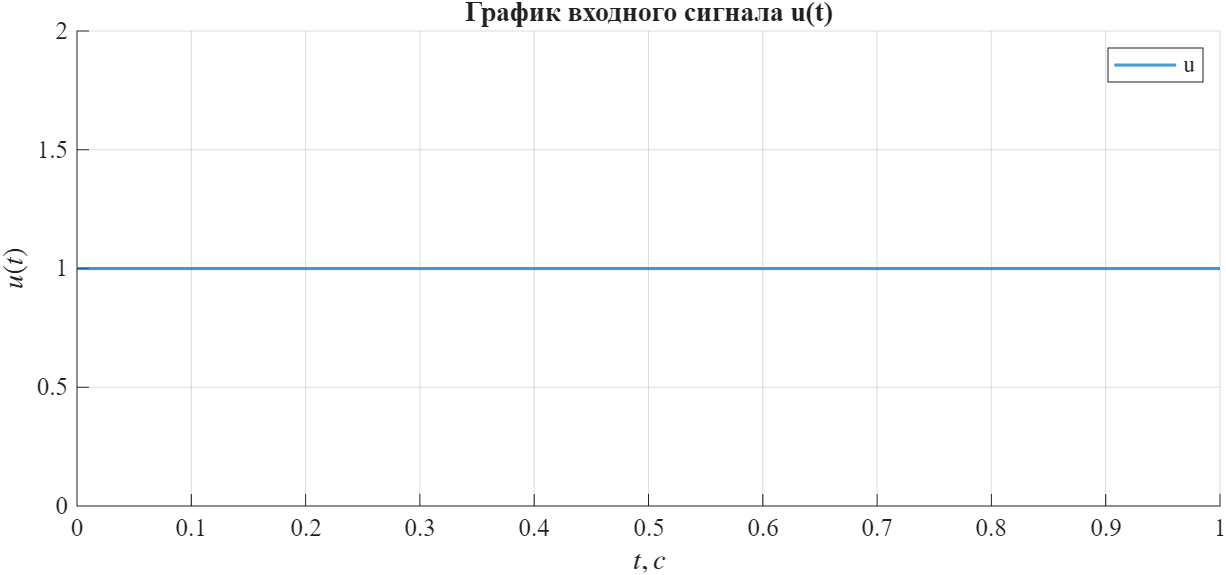
\includegraphics[width=1\linewidth]{images/Figure_1_1_2.png}
    \caption{График входного сигнала $u(t)$}
    \label{fig:placeholder}
\end{figure}

\begin{figure}[H]
    \centering
    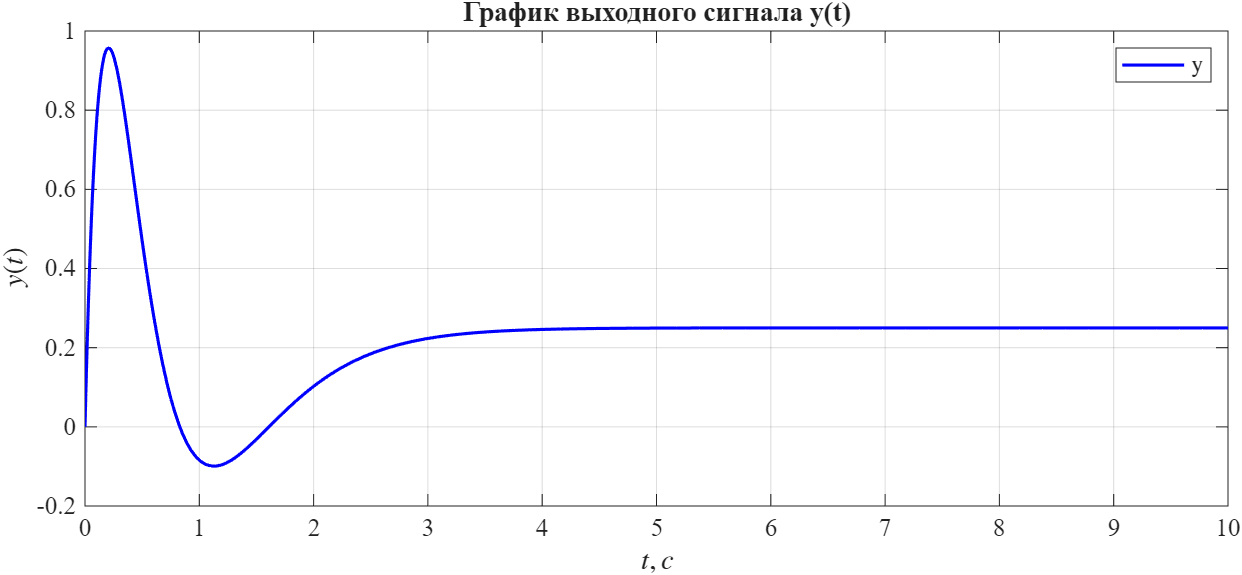
\includegraphics[width=1\linewidth]{images/Figure_1_1_1.png}
    \caption{График выходного сигнала $y(t)$}
    \label{fig:placeholder}
\end{figure}

\section{Задание 2. Переход от формы вход-выход к форме вход-состояние-выход}

\subsection{Исходные данные}
\begin{center}
\begin{tabular}{|c|c|}
\hline
Параметр & Значение \\ \hline
$a_2$ & 9 \\ \hline
$a_1$& 26 \\ \hline
$a_0$ & 24 \\ \hline
$b_2$ & 12 \\ \hline
$b_1$ & 2 \\ \hline
$b_0$ & 6 \\ \hline
\end{tabular}
\end{center}

\subsection{Математические модели системы (ПФ и представления В-С-В)}

$$
y = \dfrac{12 p^2 + 2 p + 6}{p^3 + 9 p^2 + 26 p + 24}u
$$

\textbf{Предаточная функция:}

$$
W(p)=\dfrac{12 p^2 + 2 p + 6}{p^3 + 9 p^2 + 26 p + 24}=\dfrac{19}{p+2}-\dfrac{52}{p+3}+\dfrac{45}{p+4}
$$

Перейдем к форме В-С-В

\[
\begin{cases}
    \dot x = Ax+Bu\\
    y=Cx
\end{cases}
\]

\textbf{Каноническая управляемая форма:}

$$
A=\begin{bmatrix}
    0 & 1 & 0 \\
    0 & 0 & 1 \\
    -24 & -26 & -9 \\
\end{bmatrix} \qquad B=\begin{bmatrix}
    0\\
    0\\
    1
\end{bmatrix} \qquad C=\begin{bmatrix}
    6 & 2 & 12
\end{bmatrix}
$$



\textbf{Каноническая наблюдаемая форма:}

$$
A=\begin{bmatrix}
    0 & 0 & -24 \\
    1 & 0 & -26 \\
    0 & 1 & -9 \\
\end{bmatrix} \qquad B=\begin{bmatrix}
    6\\
    2\\
    12
\end{bmatrix} \qquad C=\begin{bmatrix}
    0 & 0 & 1
\end{bmatrix}
$$

\textbf{каноническая диагональная форма:}

$$
A=\begin{bmatrix}
    -2 & 0 & 0 \\
    0 & -3 & 0 \\
    0 & 0 & -4 \\
\end{bmatrix} \qquad B=\begin{bmatrix}
    19\\
    -52\\
    45
\end{bmatrix} \qquad C=\begin{bmatrix}
    1 & 1 & 1
\end{bmatrix}
$$

\subsection{Структурные схемы системы}

\vspace{0.4cm}

\begin{figure}[H]
    \centering
\includegraphics[width=1\linewidth]{images/image_1_2_1.png}
    \caption{Структурная схема передаточной функции}
    \label{fig:placeholder}
\end{figure}

\begin{figure}[H]
    \centering
\includegraphics[width=1\linewidth]{images/image_1_2_2.png}
    \caption{Структурная схема канонической управляемой формы}
    \label{fig:placeholder}
\end{figure}
\newpage

\begin{figure}[H]
    \centering
\includegraphics[width=1\linewidth]{images/image_1_2_3.png}
    \caption{Структурная схема канонической наблюдаемой формы}
    \label{fig:placeholder}
\end{figure}

\begin{figure}[H]
    \centering
\includegraphics[width=1\linewidth]{images/image_1_2_4.png}
    \caption{Структурная схема канонической диагональной формы}
    \label{fig:placeholder}
\end{figure}

\subsection{Графики $u(t)$ и $y(t)$}

\begin{figure}[H]
    \centering
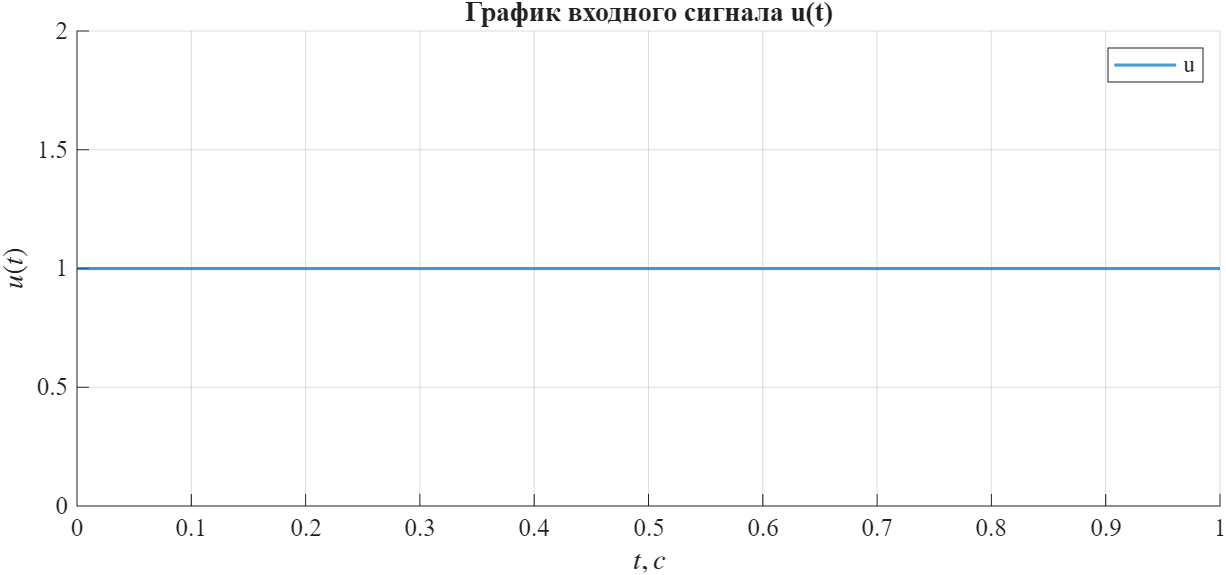
\includegraphics[width=1\linewidth]{images/Figure_1_1_2.png}
    \caption{График входного сигнала $u(t)$}
    \label{fig:placeholder}
\end{figure}

\begin{figure}[H]
    \centering
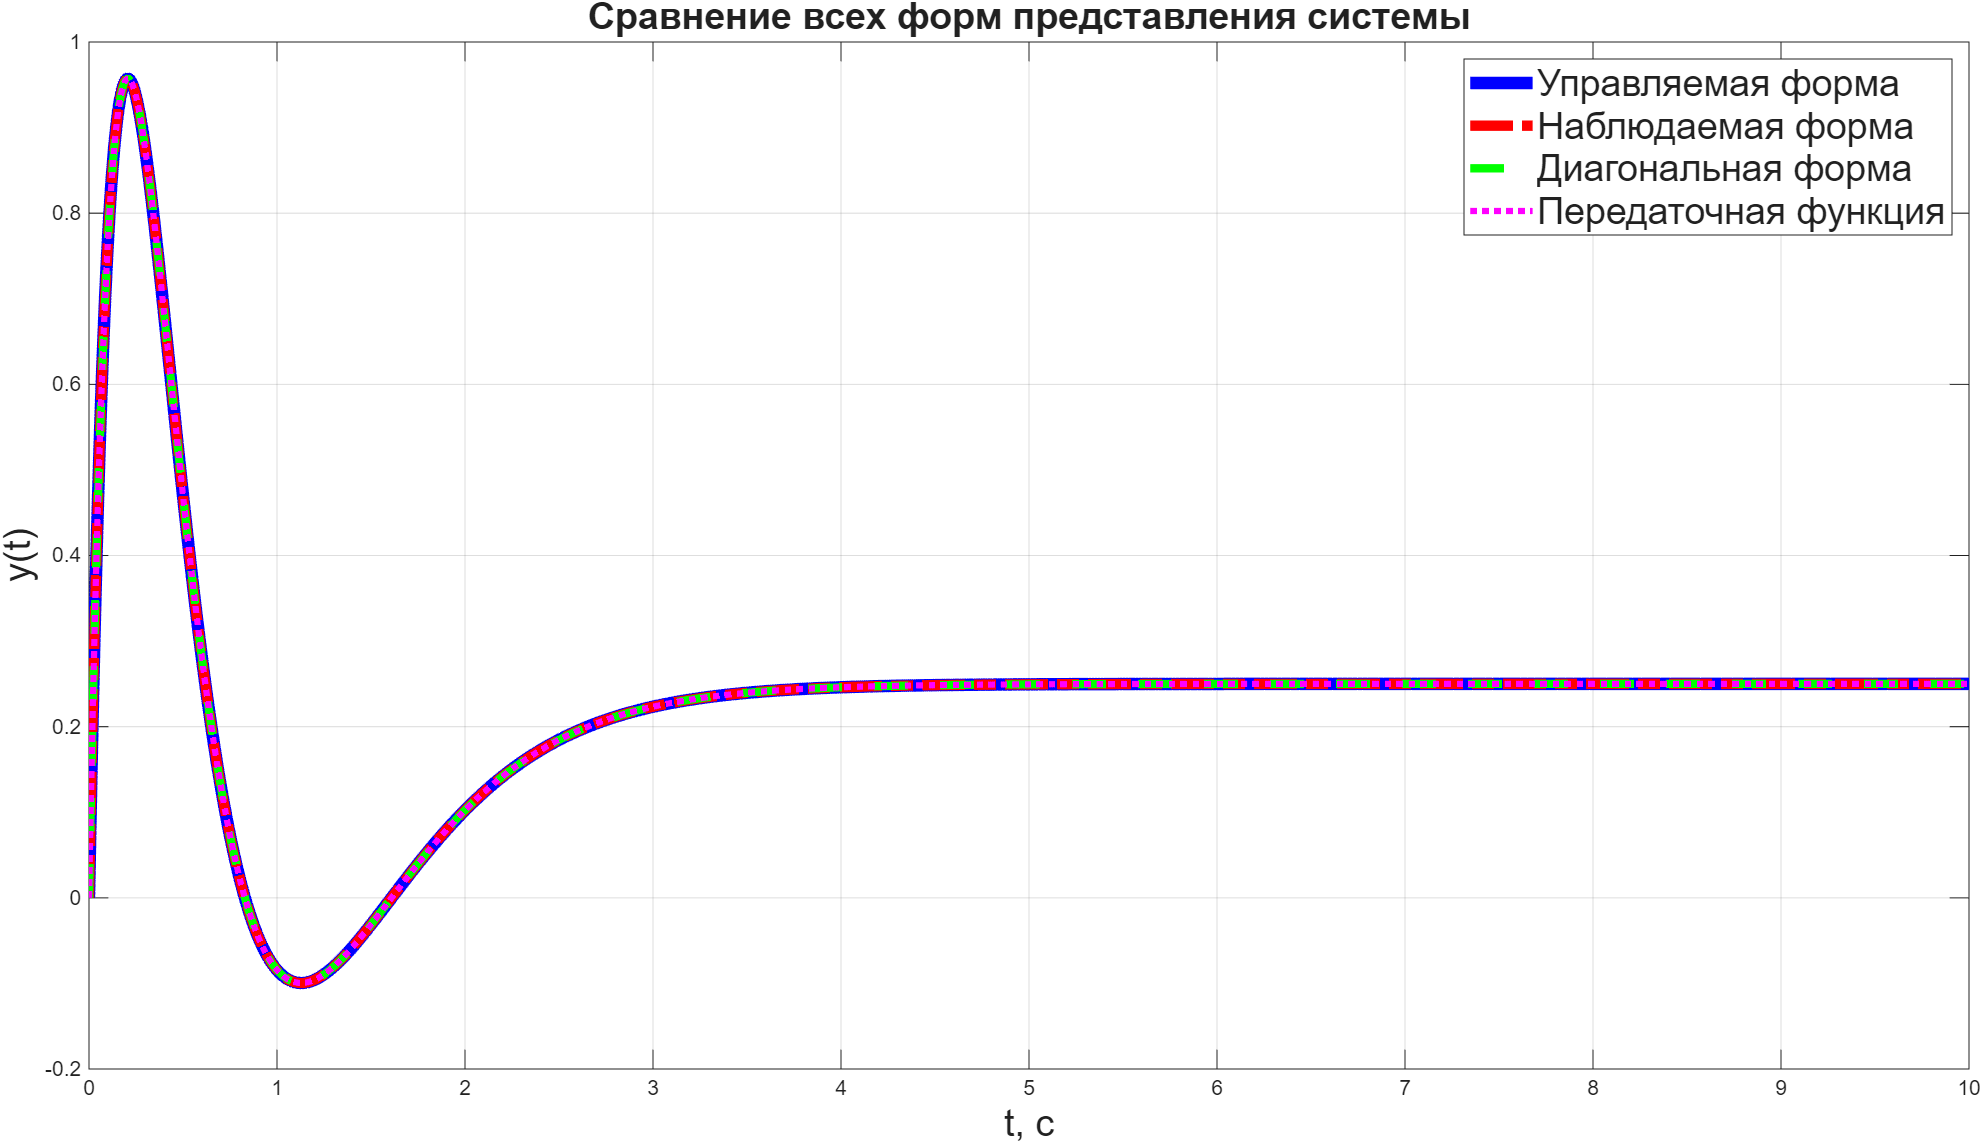
\includegraphics[width=1\linewidth]{images/Figure_1_2_1.png}
    \caption{График выходных сигналов $y(t)$ разных форм представления системы}
    \label{fig:placeholder}
\end{figure}

\subsection{Выводы:}

В ходе выполнения данного задания были получены различные формы представления линейной динамической системы: передаточная функция и три формы «вход–состояние–выход»:
\begin{itemize}
    \item каноническая управляемая форма
    \item каноническая наблюдаемая форма
    \item каноническая диагональная форма
\end{itemize}
Моделирование системы показало, что все четыре формы дают идентичные графики. Это подтверждает эквивалентность различных представлений одного и того же динамического объекта.

\section{Задание 3. Многоканальная система в форме вход-выход}

\subsection{Исходные данные}
\begin{center}
\begin{tabular}{|c|c|}
\hline
Параметр & Значение \\ \hline
$a_{11}(p)$ & p+15 \\ \hline
$a_{12}(p)$& p+3 \\ \hline
$a_{21}(p)$ & p+4 \\ \hline
$a_{22}(p)$ & p+2 \\ \hline
$b_{11}(p)$ & 7 \\ \hline
$b_{12}(p)$& 4 \\ \hline
$b_{21}(p)$ & 7 \\ \hline
$b_{22}(p)$ & 1 \\ \hline
\end{tabular}
\end{center}

\subsection{Математическая модель системы (ПМ)}

$$
A(p)y(t)=B(p)u(t)
$$
где 
$$
A(p)=\begin{bmatrix}
    p+15 &p+3\\
    p+4 &p+2
\end{bmatrix}, \qquad B(p)=\begin{bmatrix}
    7 &4\\
    7 &1
\end{bmatrix}
$$

$$
W(p)=A(p)^{-1}B(p)
$$

$$
W(p)=\begin{bmatrix}
    p+15 &p+3\\
    p+4 &p+2
\end{bmatrix}^{-1}\begin{bmatrix}
    7 &4\\
    7 &1
\end{bmatrix}=\dfrac{1}{2(5p+9)}\begin{bmatrix}
    p+2 & -p-3\\
    -p-4 &p+15
\end{bmatrix}\begin{bmatrix}
    7 &4\\
    7 &1
\end{bmatrix}
$$

$$
W(p)=\dfrac{1}{10p+18}\begin{bmatrix}
    -7 & 3p+1\\
    77 &-3p-1
\end{bmatrix}
$$

\subsection{Структурная схема системы}

\begin{figure}[H]
    \centering
    \includegraphics[width=1\linewidth]{images/image_1_3_1.png}
    \caption{Структурная схема двухканальной линейной динамической системы в форме вход-выход}
    \label{fig:placeholder}
\end{figure}

\subsection{Графики $u(t)$ и $y(t)$}

\begin{figure}[H]
    \centering
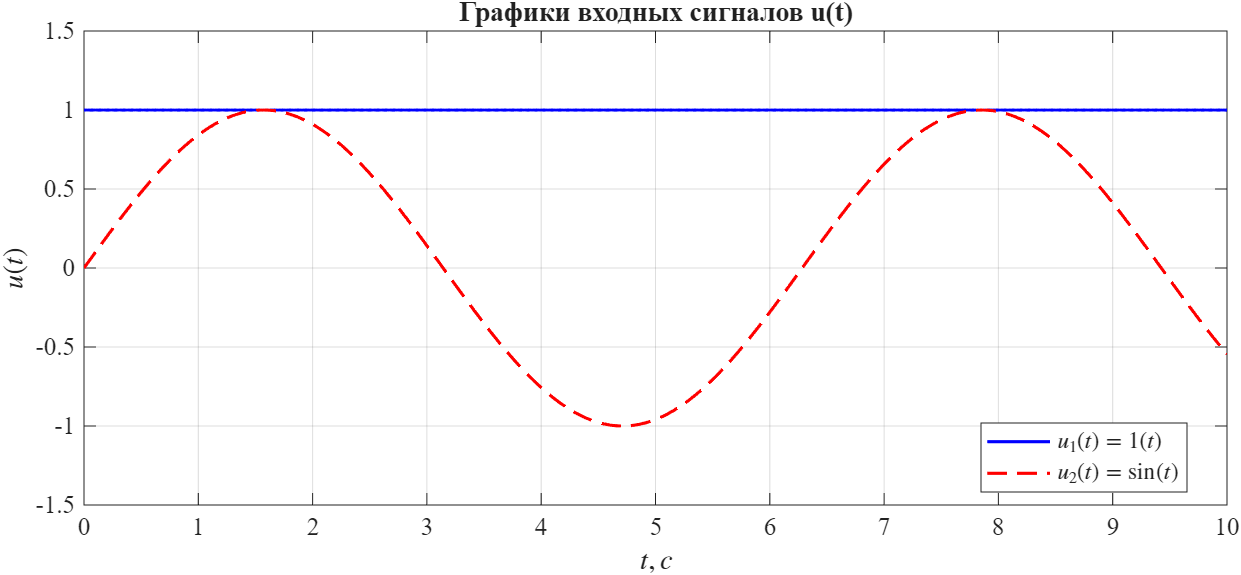
\includegraphics[width=1\linewidth]{images/Figure_1_3_1.png}
    \caption{График входных сигналов $u_1(t), \, u_2(t)$}
    \label{fig:placeholder}
\end{figure}

\begin{figure}[H]
    \centering
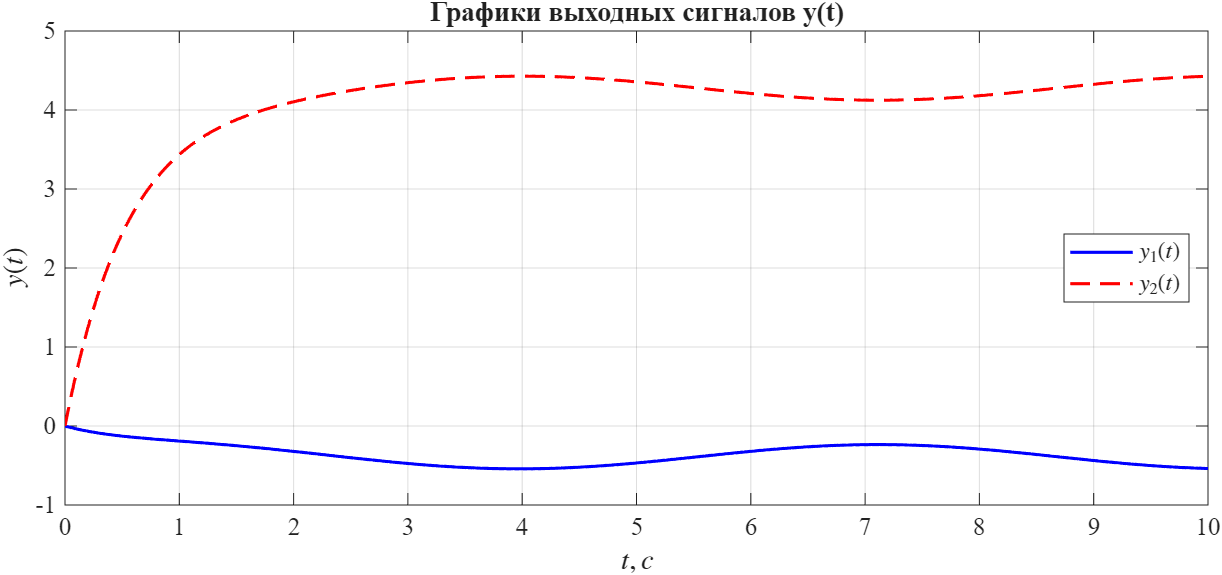
\includegraphics[width=1\linewidth]{images/Figure_1_3_2.png}
    \caption{График выходных сигналов $y_1(t), \, y_2(t)$}
    \label{fig:placeholder}
\end{figure}

\section{Задание 4. Многоканальная система в форме вход-состояние-выход}

\subsection{Исходные данные}
\begin{center}
\begin{tabular}{|c|c|}
\hline
Параметр & Значение \\ \hline
$A$ & \begin{bmatrix}
    0&-1\\
    1&-5
\end{bmatrix} \\ \hline
$B$& \begin{bmatrix}
    7&2\\
    3&5
\end{bmatrix} \\ \hline
$C$ & \begin{bmatrix}
    9&2\\
    0&3
\end{bmatrix} \\ \hline
\end{tabular}
\end{center}


\subsection{Математическая модель системы (ПМ)}

\[
\begin{cases}
    \dot x = Ax+Bu\\
    y=Cx
\end{cases}
\]
где
$$A=\begin{bmatrix}
    0&-1\\
    1&-5
\end{bmatrix}, \quad B=\begin{bmatrix}
    7&2\\
    3&5
\end{bmatrix}, \quad C=\begin{bmatrix}
    9&2\\
    0&3
\end{bmatrix}$$

\subsection{Структурная схема системы}

\begin{figure}[H]
    \centering
    \includegraphics[width=1\linewidth]{images/image_1_4_1.png}
    \caption{Структурная схема двухканальной линейной динамической системы в форме В-С-В}
    \label{fig:placeholder}
\end{figure}

\subsection{Графики $u(t)$ и $y(t)$}

\begin{figure}[H]
    \centering
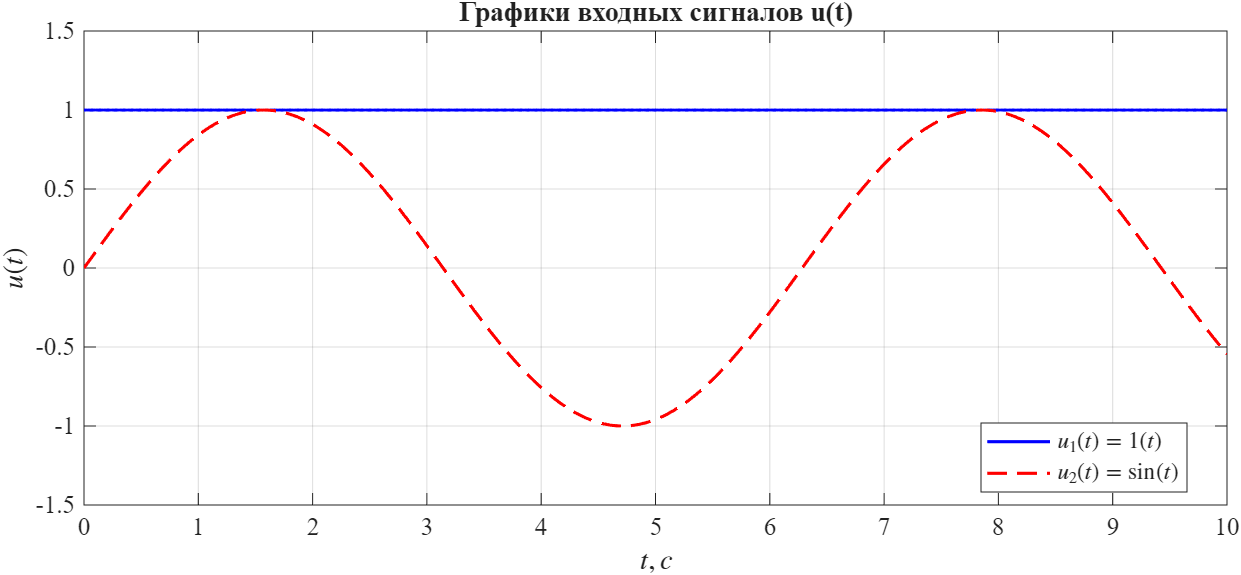
\includegraphics[width=1\linewidth]{images/Figure_1_3_1.png}
    \caption{График входных сигналов $u_1(t), \, u_2(t)$}
    \label{fig:placeholder}
\end{figure}

\begin{figure}[H]
    \centering
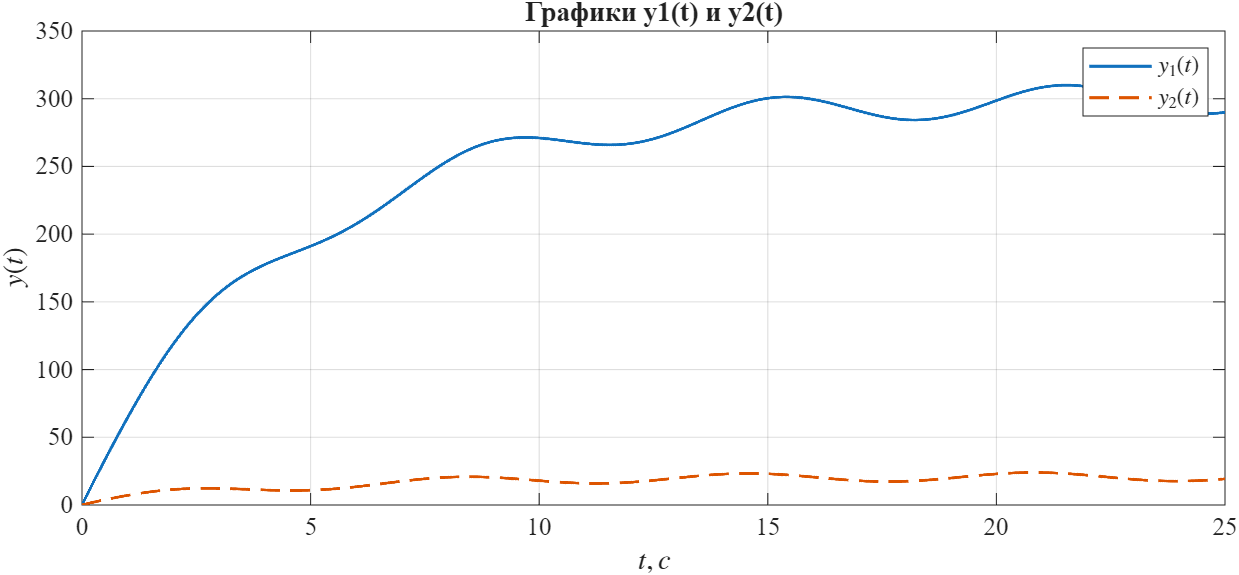
\includegraphics[width=1\linewidth]{images/Figure_1_4_1.png}
    \caption{График выходных сигналов $y_1(t), \, y_2(t)$}
    \label{fig:placeholder}
\end{figure}

\section{Выводы:}

В ходе лабораторной работы были изучены и применены на практике основные формы представления линейных динамических систем:

\begin{itemize}
    \item Форма «вход–выход» 
    \item Форма «вход–состояние–выход» (в различных канонических представлениях)
\end{itemize}

Для одноканальных и многоканальных систем были построены структурные схемы. 
Была исследована реакция на различные входные воздействия.
\end{document}